% Klassifiziert den Dokumenten-Typ
% Doku: http://exp1.fkp.physik.tu-darmstadt.de/tuddesign/
% Farben: http://www.tu-darmstadt.de/media/medien_stabsstelle_km/services/medien_cd/das_bild_der_tu_darmstadt.pdf
%  bigchapter: Chapter haben doppelte Schriftgröße
%  linedtoc: Linien im Inhaltsverzeichnis wie bei Überschriften
%  colorbacktitle: Der Dokumenten-Titel wird mir der Accentfarbe hinterlegt
\documentclass[bigchapter,colorback,accentcolor=tud4b,linedtoc,11pt]{tudreport}

% Input Dokument hat das Encoding UTF-8
\usepackage[utf8]{inputenc}
% Wichtiges Paket für Links und verlinktes Inhaltsverzeichnis
\usepackage[ngerman]{hyperref}
% Paket für Fußnoten
\usepackage[stable]{footmisc}
% Paket für amsmath (aligned mathe formeln)
\usepackage{amsmath}
% Paket für Bibliotheks-Verzeichnis, square: Verwende eckige statt runde klammern
% \usepackage[square]{natbib}
% Paket zum Plotten von Datensätzen
\usepackage{pgfplots}
\usepgfplotslibrary{patchplots}


\pgfkeys{%
  /pgfplots/seperators/.style={%
    /pgf/number format/use comma
  }
}

% Anhänge für Original-Messdaten
\usepackage{fancyvrb}

% redefine \VerbatimInput
\RecustomVerbatimCommand{\VerbatimInput}{VerbatimInput}%
{fontsize=\footnotesize,
 %
 frame=lines,  % top and bottom rule only
 framesep=2em, % separation between frame and text
 fontsize=\scriptsize,
 %
 labelposition=topline,
 %
 commandchars=\|\(\), % escape character and argument delimiters for
                      % commands within the verbatim
 commentchar=*        % comment character
}

% Polar Plots
\usetikzlibrary{pgfplots.polar}
% Verwende deutsche Bezeichner für Inhaltsverzeichnis, ... (ngerman = New German: neue Rechtschreibung)
\usepackage{ngerman}
% Deutsche Zahlen (entfernt z.B. das Leerzeichen nach einem Dezimal-Komma)
\usepackage{ziffer} 

\usepackage[verbose]{placeins}

%wegen Grafikverschiebung hinzugefügt
\usepackage{float}

%\usepackage{graphicx}
%\usepackage{caption}
\usepackage{subcaption} %Für subfigures

% PDF-Optionen
\hypersetup{%
  pdftitle={TU Darmstadt \- Physikalisches Praktikum für Fortgeschrittene},
  pdfauthor={Esra Bauer und Sören Link},
  pdfsubject={Versuch 4.4B},
  pdfview=FitH,
}
% Nummeriere formeln in Subsections einzeln
% Kleines makro zur assymetrischen Fehlerangabe

% Entspricht-Zeichen
\usepackage{scalerel}

\newcommand\equalhat{%
\let\savearraystretch\arraystretch
\renewcommand\arraystretch{0.3}
\begin{array}{c}
\stretchto{
    \scalerel*[\widthof{=}]{\wedge}
    {\rule{1ex}{3ex}}%
}{0.5ex}\\ 
=%
\end{array}
\let\arraystretch\savearraystretch
}
%BEGINN TITELSEITE

\title{Holographie}

\subtitle{Esra Bauer (1906093) \\Sören Link}

\subsubtitle{Betreuer: Stefan Breuer \hfill Versuchsdatum: 11. Mai 2015}

\author{Esra Bauer, Sören Link}

%\settitlepicture{img/title.jpg}

\institution{Physikalisches Praktikum \\für Fortgeschrittene \\ Versuch 4.4B}

\date{\today}


%ENDE TITELSEITE

\begin{document}
%ANFANG DOKUMENT

%Titelseite einfügen
\maketitle

%Inhaltsverzeichnis einfügen
\tableofcontents

%ANFANG INHALT

\chapter{Einleitung}

In diesem Versuch wird das Abbildungsverfahren der Holographie untersucht und praktisch angewendet. Es werden sowohl die benötigen Chemikalien hergestellt als auch ein holographisches Gitter, Punkt- und Objekthologramme hergestellt und rekonstruiert sowie der theoretische Hintergrund beleuchtet und z.B. das holographische Abbildungsgesetz mithilfe des Punkthologramms überprüft. Holographie besitzt vielfältige Anwendungen, die von holographisch-optischen Bauelementen ( u.a. in Barcodescannern, Laserscannern und Head-up-Displays) über holographische Endoskopie in der Medizin bis hin zu künstlerischen Zwecken reichen.

\chapter{Grundlagen}

\section{Helium-Neon-Laser}

\section{Grundlagen der Holographie}

\subsection{Aufnahme eines Hologramms}

\subsection{Rekonstruktion eines Hologramms}

\chapter{Durchführung}

\section{Vorbereitung der Photochemikalien}

Zur Erzeugung der Hologramme werden ein Entwicklerbad, ein Bleichbad sowie zwei Schalen mit destilliertem Wasser benötigt. Entwickler- und Bleichflüssigkeit werden gemäß der im Versuch ausliegenden Tabellen mit destilliertem Wasser angesetzt, wobei Schutzhandschuhe und -kleidung zu tragen sind. Anschließend werden vier Glasschalen aufgestellt, von denen die erste mit Entwicklerflüssigkeit, die zweite und vierte mit destilliertem Wasser und die dritte mit Bleichflüssigkeit gefüllt werden. So kann die Entwicklung später im Dunkeln sicher durchgeführt werden.

\section{Justage des Raumfilters}

Bestehend aus einem Mikroskopobjektiv (Numerische Apertur NA = 0,85), einer Lochblende mit 54 µm Durchmesser sowie einer Linse der Brennweite f = 25 cm, wird der Raumfilter in den Strahlengang des Lasers gebracht, so dass der Brennpunkt des aus dem Mikroskopobjektivs austretenden Stahls genau in der Blende liegt und mit dem Brennpunkt der Linse zusammenfällt. Der aus der Blende austretende divergente Strahl wird mittels der Linse gebündelt, wobei mittels eines auf einem Schirm gezeichneten Fadenkreuzes der Strahl ausgerichtet werden konnte und überprüft wurde, dass der Strahldurchmesser in einem Abstand bis etwa 2 Meter konstant 4 cm beträgt.

\begin{figure}[H]
\centering
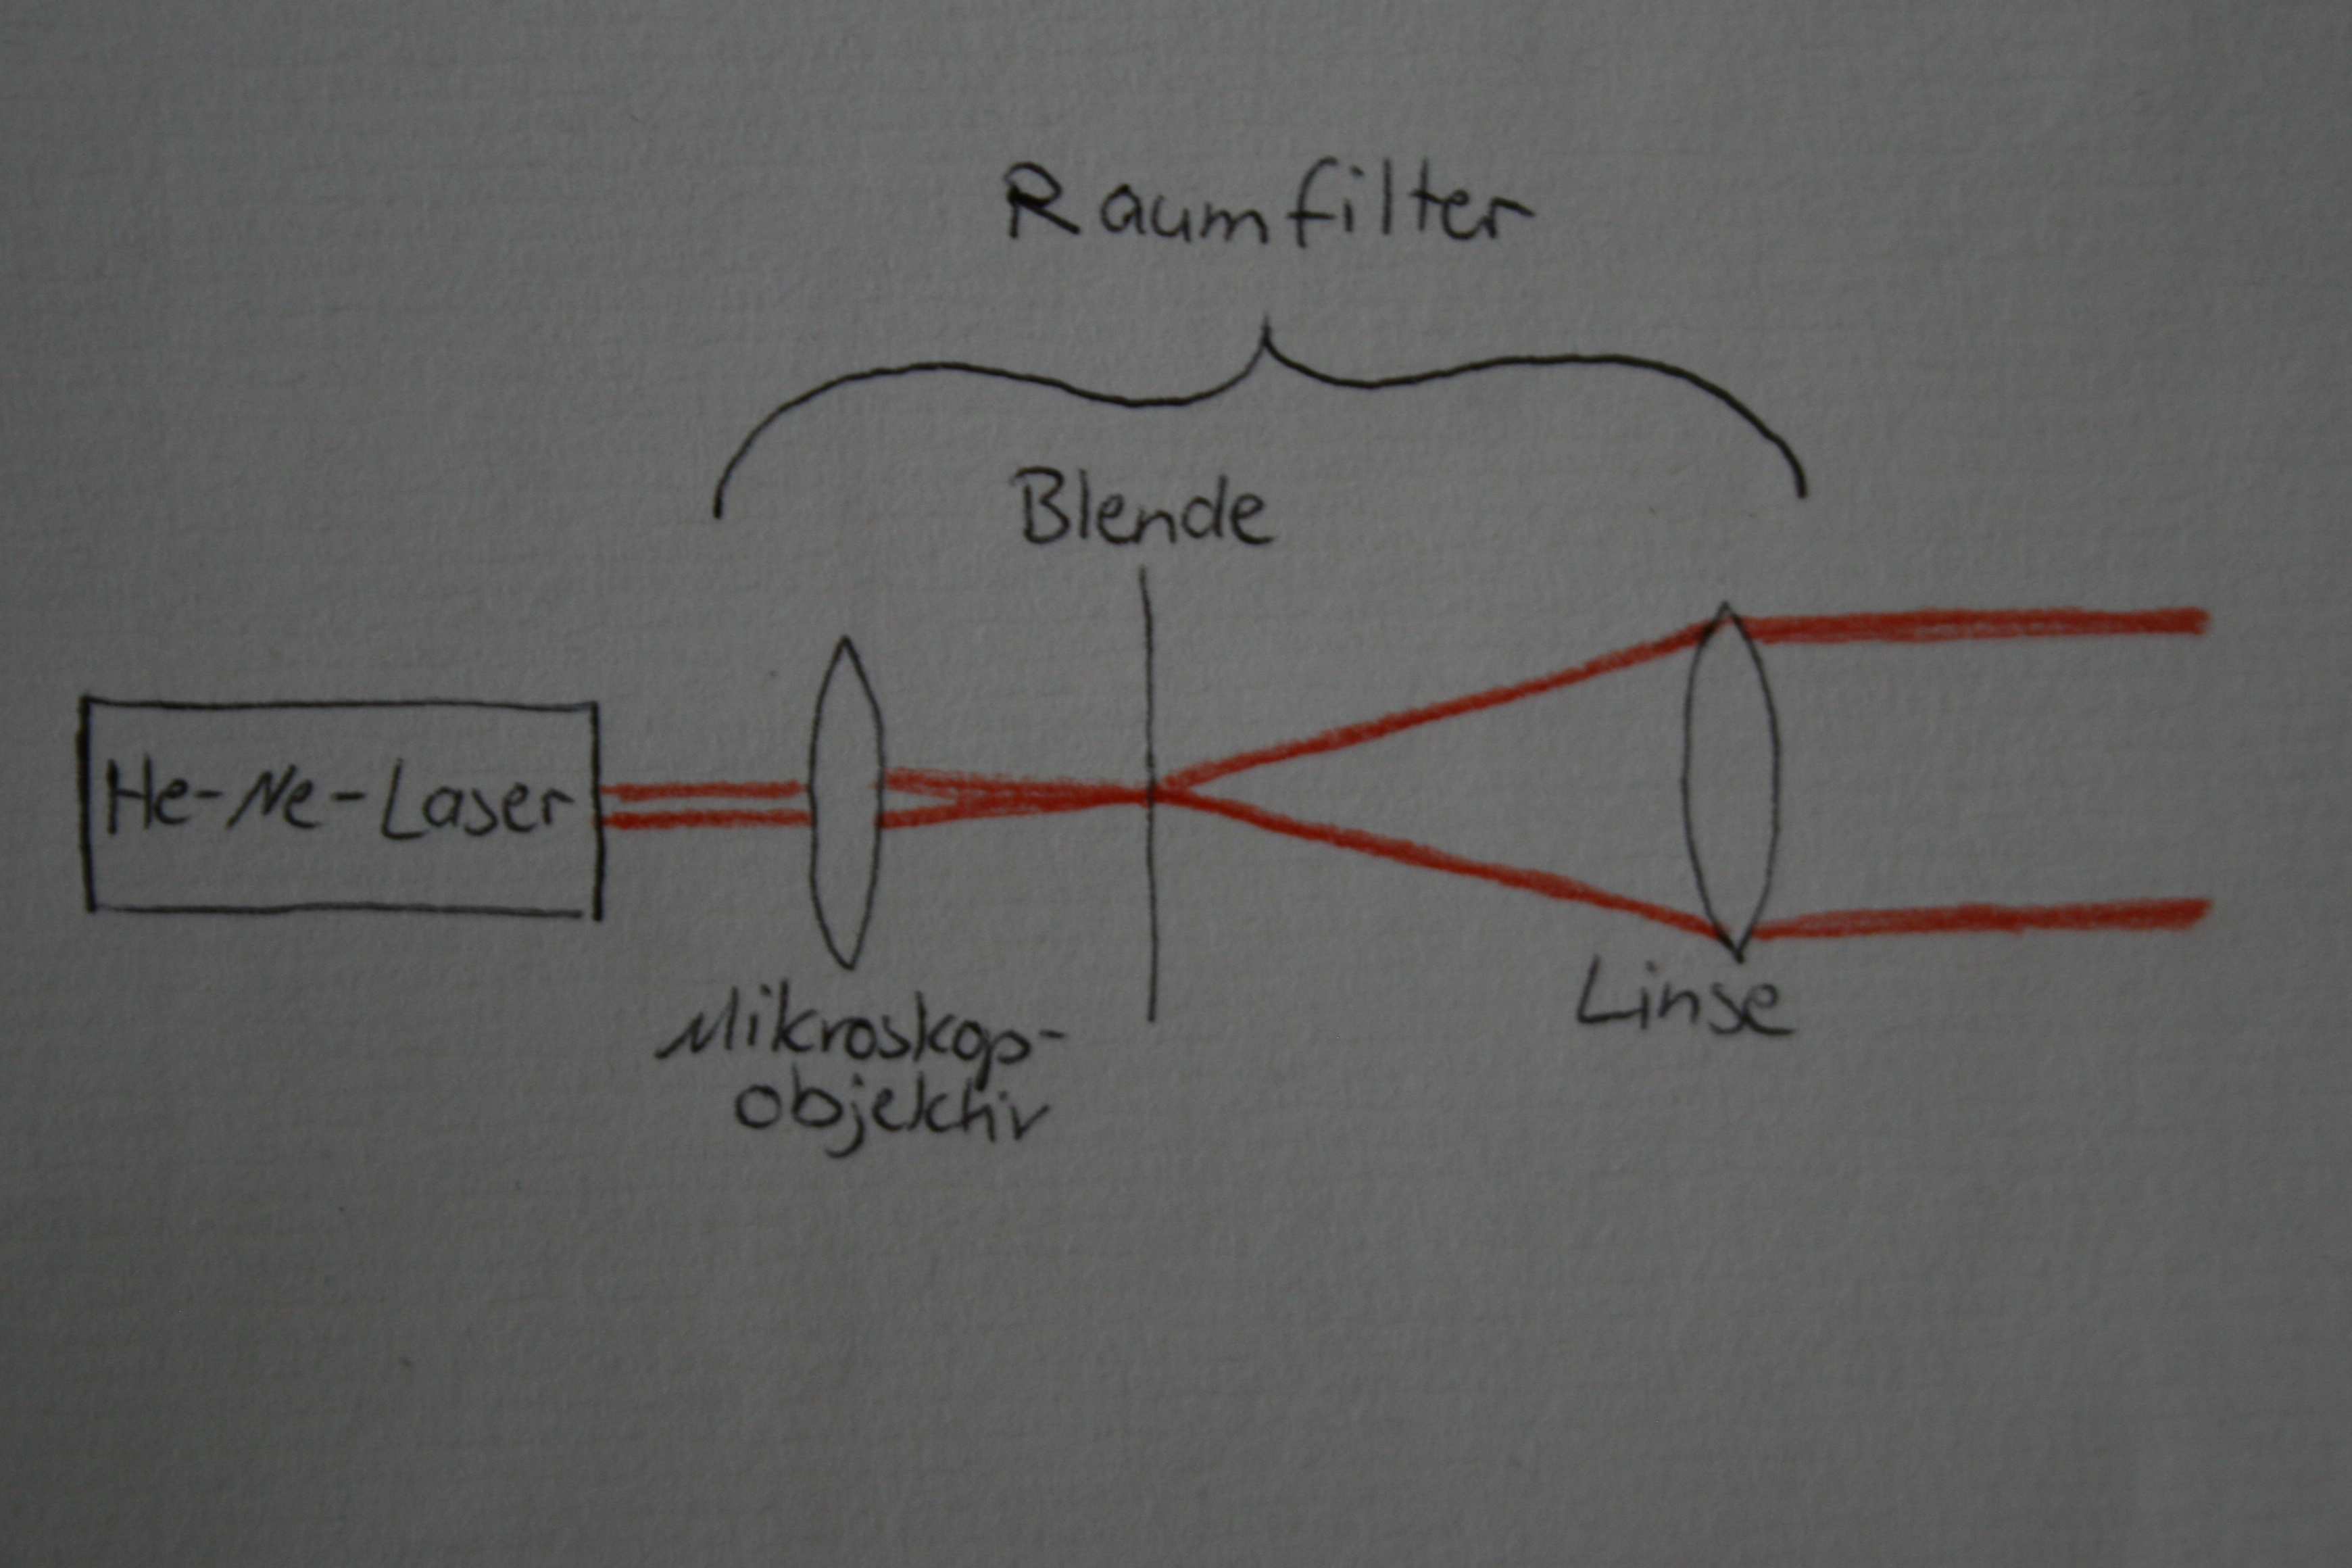
\includegraphics[width=130mm]{img/Raumfilter.JPG}
\caption{Aufbau des Raumfilters}
\end{figure}

\section{Erzeugung eines holographischen Gitters}

Nachdem der Raumfilter justiert ist, wird in einem Abstand von etwa 70 cm zur Sammellinse ein Strahlteiler in den Strahlengang eingebracht, mit dem der Laserstrahl in zwei Teilstrahlen möglichst gleicher Intensität aufgeteilt wird. In den Photoplattenhalter wird Papier eingelegt, um die Justage des Strahls zu ermöglichen. Weiterhin steht ein einstellbarer Spiegel zur Verfügung, mittels dessen der durch den Strahlteiler abgelenkte Teilstrahl wieder zurück auf den Photoplattenhalter, resp. das Justagepapier geleitet wird, so dass beide Strahlen deckungsgleich aufeinandertreffen. Mit bloßem Auge lässt sich hier noch nichts erkennen, jedoch sehen wir, wenn das Justagepapier entfernt wird, mithilfe einer Vergrößerungsapparatur bereits Interferenzstreifen, die auch mittels der zur Verfügung stehenden CCD-Kamera und des Bildschirms gut beobachtbar sind. Wird einer der Teilstrahlen blockiert, verschwindet das Interferenzmuster.

Im nächsten Schritt kann also das Hologramm aufgenommen werden. Dazu müssen Belichtungs- und Entwicklungszeiten usw. genau eingehalten werden, daher verwenden wir eine Stoppuhr und arbeiten zu viert, wodurch ein reibungsloser Ablauf gewährleistet ist. Nach Abdunklung des Raums kann die lichtdichte Box geöffnet, eine Photoplatte entnommen und in den Photoplattenhalter eingesetzt werden. Die Box wird geschlossen und nach kurzer Wartezeit wird die Belichtung gestartet und nach genau 20 s beendet. Danach entnehmen wir die Photoplatte und schwenken sie zuerst für 2 Minuten im Entwicklerbad und dann für eine Minute im Bleichbad, wodurch die Entwicklung gestoppt wird. Nun kann das Licht bereits wieder eingeschaltet werden; die Photoplatte wird jedoch nochmals im Bleichbad geschwenkt, bis die dunkle Schicht komplett aufgehellt ist. Hierbei werden die belichteten Anteile in lösliche Silbersalze umgewandelt und ausgewaschen. Das Hologramm wird dadurch heller. Sind alle Bereiche der Photoplatte transparent, wird sie für 5 Minuten im letzten Wasserbad geschwenkt und anschließend nochmals mit destilliertem Wasser gespült und in senkrechter Position mit einem Ventilator getrocknet. Anschließend kann das Hologramm wieder in den Strahlengang gebracht und rekonstruiert werden, indem der Strahlteiler entfernt wird bzw. der Objektstrahl blockiert wird. Es werden Punkte im typischen Interferenzmuster sichtbar, jeweils unter einem bestimmten positiven und negativen Winkel zur Photoplatte.

\section{Hologramm eines Punktes}

Um das Hologramm eines Punktes aufnehmen zu können, bringen wir eine weitere Linse in den abgezweigten Strahlengang zwischen Spiegel und Photoplattenhalter, derart dass der Strahldurchmesser am Ort der Photoplatte wieder 4 cm beträgt. D.h. der Brennpunkt der Linse stellt die Punktlichtquelle dar und liegt im abgezweigten Strahlengang. Sobald die Einstellungen beendet sind, kann wieder wie im vorherigen Abschnitt beschrieben belichtet und entwickelt werden. Bei der Rekonstruktion lassen sich zwei überaus helle Punkte beobachten, wieder jeweils unter positivem und negativem Winkel.

Um später das holographische Abbildungsgesetz verifizieren zu können, muss die Bildweite in Abhängigkeit des Krümmungsradius der Rekonstruktionswelle gemessen werden. Dazu wird zunächst ein Schirm hinter den Photoplattenhalter, in welchem das Punkthologramm eingesetzt ist, aufgestellt, auf dem dadurch der Punkt sichtbar wird. Nun wird eine zusätzliche Linse in den Strahlengang zwischen Sammellinse und Punkthologramm gebracht, mittels derer wir durch Verschiebung verschiedene Krümmungsradien erzeugen können. Der Schirm wird nach jeder Verschiebung der Linse so positioniert, dass der Punkt scharf abgebildet wird, anschließend kann die Bildweite direkt als Abstand zwischen Schirm und Punkthologramm gemessen werden.

\section{Objektholographie}

\chapter{Auswertung}

\section{Raumfilter und He-Ne-Laser}

Die Funktion des Raumfilters lässt sich in drei Bereiche gliedern: Zum einen wird der Strahldurchmesser auf das benötigte Maß von etwa 4 cm aufgeweitet, da der Laser mit einem Strahldurchmesser von lediglich 1-2 mm emittiert. Zum andern wird die Dispersion der Linsen ausgenutzt, um infrarotes Licht herauszufiltern. Dadurch, dass infrarotes Licht weniger stark gebrochen wird, kann es nämlich nicht durch die Blende gelangen, die in den Brennpunkt für den erwünschten sichtbaren Anteil positioniert wird. Zudem absorbieren die Linsen einen Teil des infraroten Lichtes, welches somit insgesamt sehr effektiv herausgefiltert wird. Zuletzt wirkt der Raumfilter als Beugungsordnungsfilter. Durch die sehr geringe Größe der Blende von 54 µm wird die Raumunschärfe des Laserstrahls gering (deswegen heißt der Raumfilter Raumfilter), wodurch nach der Heisenbergsche Unschärferelation die Impulsunschärfe zunimmt, was in einer Glättung bzw. Homogenisierung des Lichtstrahls resultiert. Dadurch werden die negativen Auswirkungen durch eventuell verschmutzte Linsen auf die Kohärenz verringert und im Idealfall gelangt von den verschiedenen räumlich getrennten Beugungsordnungen nur die 0. durch den Raumfilter. Die tatsächliche Anzahl der transmittierten Beugungsordnungen wird im Folgenden berechnet.

Ausgehend von der Beugung an einer Lochblende ergibt sich hinter der Blende die Intensitätsverteilung

$$I(\theta) = I_0 \left[ \frac{2 J_1(x(\theta))}{x(\theta)} \right]^2,$$

wobei $\theta$ der Winkel und $J_1$ die Besselfunktion erster Ordnung ist. Mit dem Durchmesser R der Lochblende erhält man $x(\theta)$ aus folgender Gleichung: 

$$x(\theta) = \frac{2 \pi R}{\lambda} sin(\theta).$$

Um die höchste Beugungsordnung zu ermitteln, betrachten wir den Sinus des maximalen Winkels, also

$$sin(\theta_{max}) = \frac{0,5 D}{\sqrt{(0,5 D)^2 + f^2}},$$

mit dem Strahldurchmesser D = 4 cm und der Brennweite bzw. dem Abstand der Linse zur Lochblende f = 25 cm. Setzt man $\lambda = 632,8~nm$ ein, ergibt sich der maximale Wert zu $x_{max} = 13,61 \pi$.

Nun betrachten wir die Nullstellen der Besselfunktion, da diese die Intensitätsminima und somit die Zahl der Beugungsordnungen angeben. Die Nullstellen lauten: 

\begin{center}
$x_1 = 1,22 \pi$ \\
$x_2 = 2,23 \pi$ \\
$x_3 = 3,24 \pi$ \\
$x_4 = 4,24 \pi$ \\
$x_5 = 5,24 \pi$ \\
$x_6 = 6,24 \pi$ \\
$x_7 = 7,24 \pi$ \\
$x_8 = 8,24 \pi$ \\
$x_9 = 9,25 \pi$ \\
$x_{10} = 10,25 \pi$ \\
$x_{11} = 11,25 \pi$ \\
$x_{12} = 12,25 \pi$ \\
$x_{13} = 13,25 \pi$ \\
$x_{14} = 14,25 \pi$
\end{center}

Somit ergibt sich im Vergleich mit $x_{max}$, dass 13 Minima auftreten, dies entspricht 12 Beugungsordnungen. Von dem Idealzustand, dass lediglich die nullte Beugungsordnung im austretenden Strahl enthalten ist, kann also keine Rede sein.

\section{Holographisches Gitter}

\section{Punktholographie}

\section{Objektholographie}

\chapter{Fazit}

%ENDE INHALT
\cleardoublepage{}
% Eintrag fürs Inhaltsverzeichnis
\newpage
\begin{thebibliography}{100}
%  \bibitem{anleitung} Versuchsanleitung Magnetfeldmessung, heruntergeladen am 15.2.2015 von der Homepage des IKP der TU Darmstadt
\end{thebibliography}
\end{document}

%%% Local Variables:
%%% mode: latex
%%% TeX-master: t
%%% End:
